%\documentclass{beamer}
\documentclass[handout]{beamer}
%\documentclass{article}
\usepackage{amsmath}
\usepackage{array}
\usepackage{graphicx}
\usepackage{multirow}
\setbeamertemplate{navigation symbols}{}
\setbeamertemplate{caption}{\insertcaption} \setbeamertemplate{caption label separator}{}
\renewcommand{\emph}{\textbf}
\usetheme{Warsaw}
\title{Ch. 9 -- Inferences Based on Two Samples}
%\setlength{\parskip}{.2cm}
\DeclareMathOperator{\Bin}{Bin}
\DeclareMathOperator{\Cov}{Cov}
\DeclareMathOperator{\Corr}{Corr}

\begin{document}
\begin{frame}
\begin{beamercolorbox}[rounded=true,wd=\textwidth,center]{title}
\usebeamerfont{title}\inserttitle
\end{beamercolorbox}
\end{frame} 

\begin{frame}{Two-sample z Test}
Suppose we are given two independent normal random samples:
\begin{itemize}
\item $X_1,\dots,X_m$ from a $N(\mu_1,\sigma_1^2)$ distribution
\item $Y_1,\dots,Y_n$ from a $N(\mu_2,\sigma_2^2)$ distribution
\end{itemize}
\pause If we know the variances $\sigma_1^2$ and $\sigma_2^2$, we may use a \emph{two-sample z test} to test the null hypothesis $H_0: \mu_1-\mu_2 = \Delta_0$:

\pause\begin{block}{}
\begin{tabular}{c|c|c}
Test Statistic & Alternative hypothesis & Rejection region \\ \hline
\multirow{3}{*}{$\displaystyle Z=\frac{\overline X-\overline Y-\Delta_0}{\sqrt{\frac{\sigma_1^2}m+\frac{\sigma_2^2}n}}$} & $H_a: \mu_1-\mu_2>\Delta_0$ & $Z>z_{\alpha}$ \\
& $H_a: \mu_1-\mu_2<\Delta_0$ & $Z<-z_{\alpha}$ \\
& $H_a: \mu_1-\mu_2\neq\Delta_0$ & $|Z|>z_{\alpha/2}$\\
\end{tabular}
\end{block}

\pause If $m$ and $n$ are large (say, $m>40$ and $n>40$), then we may use sample variances $S_1^2$ and $S_2^2$ in place of $\sigma_1^2$ and $\sigma_2^2$ and may drop the assumption that the distributions are normal.
\end{frame}

\begin{frame}{Example}
\begin{block}{}
A random sample of 20 specimens of cold-rolled steel had an average yield strength of 29.8 ksi. For a random sample of 25 two-sided galvanized steel specimens the average was 34.7 ksi. Assuming that the two yield-strength distributions are normal with $\sigma_1=4.0$ and $\sigma_2=5.0$, does the data provide significance evidence (at the $\alpha=.01$ level) for a difference between the mean yield strength of the two types of specimens?
\end{block}

\pause We want to test the null hypothesis $H_0: \mu_1-\mu_2=0$ against the alternative $H_a: \mu_1-\mu_2\neq 0$. \pause We calculate the test statistic:
$$Z=\frac{\overline X-\overline Y-\Delta_0}{\sqrt{\frac{\sigma_1^2}m+\frac{\sigma_2^2}n}}
\uncover<3->{= \frac{29.8-34.7-0}{\sqrt{\frac{(4.0)^2}{20}+\frac{(5.0)^2}{25}}}}
\uncover<4->{=-3.65}$$

\uncover<5->{The P-value for the test is $P(|Z|>3.65)=2\Phi(-3.65)=.00026$.}
\uncover<6->{This provides strong evidence for a difference in the mean yield strengths of the two types of specimens.}
\end{frame}

\begin{frame}{z Confidence Interval for Difference of Two Means}
Suppose we are given two independent normal random samples:
\begin{itemize}
\item $X_1,\dots,X_m$ from a $N(\mu_1,\sigma_1^2)$ distribution
\item $Y_1,\dots,Y_n$ from a $N(\mu_2,\sigma_2^2)$ distribution
\end{itemize}
\pause Assume we know the variances $\sigma_1^2$ and $\sigma_2^2$.
\pause \begin{block}{}
A $100(1-\alpha)\%$ confidence interval for $\mu_1-\mu_2$ is given by
$$\overline{X} - \overline{Y} \pm z_{\alpha/2}\sqrt{\frac{\sigma_1^2}m+\frac{\sigma_2^2}n}$$
\end{block}
\pause If $m$ and $n$ are large (say, $m>40$ and $n>40$), then we may use sample variances $S_1^2$ and $S_2^2$ in place of $\sigma_1^2$ and $\sigma_2^2$ and may drop the assumption that the distributions are normal.
\end{frame}

\begin{frame}{Example}
\begin{block}{}
A random sample of 20 specimens of cold-rolled steel had an average yield strength of 29.8 ksi. For a random sample of 25 two-sided galvanized steel specimens the average was 34.7 ksi. Assuming that the two yield-strength distributions are normal with $\sigma_1=4.0$ and $\sigma_2=5.0$, find a 95\% confidence interval for the difference in mean yield strength between the two types of specimens?
\end{block}

\pause
\begin{align*}
&\overline{X} - \overline{Y} \pm z_{\alpha/2}\sqrt{\frac{\sigma_1^2}m+\frac{\sigma_2^2}n}\\
\uncover<3->{&= 29.8 - 34.7 \pm 1.96\sqrt{\frac{(4.0)^2}{20}+\frac{(5.0)^2}{25}}}\\
\uncover<4->{&= -4.9 \pm  2.63}
\end{align*}
\end{frame}

\begin{frame}{Two-Sample t Test (Welch's t Test)}
Suppose we are given two independent normal random samples:
\begin{itemize}
\item $X_1,\dots,X_m$ from a $N(\mu_1,\sigma_1^2)$ distribution
\item $Y_1,\dots,Y_n$ from a $N(\mu_2,\sigma_2^2)$ distribution
\end{itemize}
\pause If we don't know the variances $\sigma_1^2$ and $\sigma_2^2$, we may use a \emph{two-sample t test} to test the null hypothesis $H_0: \mu_1-\mu_2 = \Delta_0$:

\begin{block}{}
\begin{tabular}{c|c|c}
Test Statistic & Alternative hypothesis & Rejection region \\ \hline
\multirow{3}{*}{$\displaystyle T=\frac{\overline X-\overline Y-\Delta_0}{\sqrt{\frac{S_1^2}m+\frac{S_2^2}n}}$} & $H_a: \mu_1-\mu_2>\Delta_0$ & $T>t_{\alpha,\nu}$ \\
& $H_a: \mu_1-\mu_2<\Delta_0$ & $T<-t_{\alpha,\nu}$ \\
& $H_a: \mu_1-\mu_2\neq\Delta_0$ & $|T|>t_{\alpha/2,\nu}$\\
\end{tabular}
\end{block}

\pause
Here the degrees of freedom $\nu$ is estimated by
$$\nu = \frac{\displaystyle \left(\frac{S_1^2}{m}+\frac{S_2^2}n\right)^2}{\displaystyle\frac{(S_1^2/m)^2}{m-1}+\frac{(S_2^2/n)^2}{n-1}}$$
\end{frame}

\begin{frame}{Example}
The deterioration of many municipal pipeline networks across the country is a growing concern. One technology proposed for pipeline rehabilitation uses a flexible liner
threaded through existing pipe. An article reported the following data on tensile strength (psi) of liner specimens both when a certain fusion process was used and when this process was not used:

\begin{center}
\begin{tabular}{l|p{9cm}}
No fusion &
2748
3149
2700
2655
2822
2511
3257
3213
3220
2753
\\ \hline
Fusion &
3027
3356
3359
3297
3125
2910
2889
2902
\end{tabular}
\end{center}
%pdf("ch9_dotplot.pdf",height=2,width=9);
%par(mai=c(.5,1,0,0)+.05,omi=c(0,0,0,0)+.05,xpd=TRUE,las=1);
%stripchart(list(nofus,fus),pch=19,at=1:2/3,ylim=c(0.25,.75),group.names=list("No fusion","Fusion"))
%#stripchart(nofus,pch=19,xlim=c(2500,3400),add=TRUE,col="red",at=1)
%dev.off();

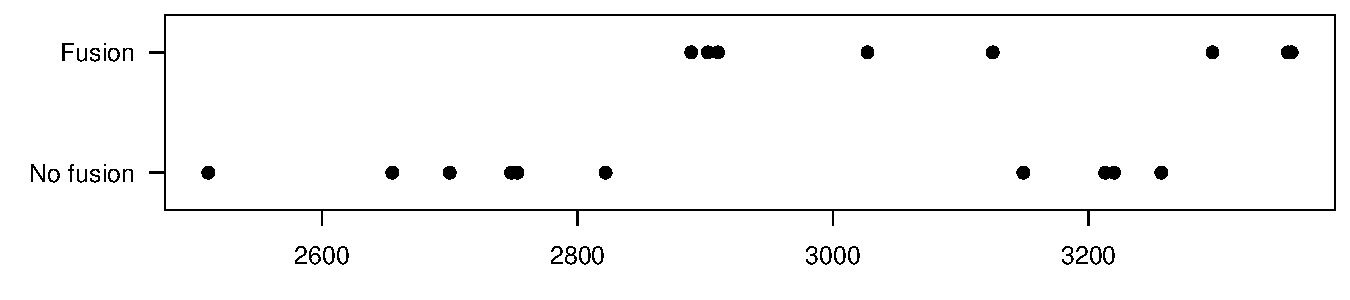
\includegraphics[scale=.5]{ch9_dotplot.pdf}
\end{frame}

\begin{frame}{Example}
\begin{block}{}
Does the data provide significant evidence for a difference in the mean tensile strength of the two types of specimens?
\end{block}

%\vspace{-.5cm}
%\begin{center}
%\begin{tabular}{l|p{9cm}}
%No fusion &
%2748
%3149
%2700
%2655
%2822
%2511
%3257
%3213
%3220
%2753
%\\ \hline
%Fusion &
%3027
%3356
%3359
%3297
%3125
%2910
%2889
%2902
%\end{tabular}
%\end{center}
%
\pause We will test the null hypothesis $H_0: \mu_1-\mu_2=0$ against the alternative $H_a: \mu_1-\mu_2\neq 0$. 

\pause The specimens with no fusion have $\overline X=2902.8$ and $S_1=277.3$, while those with fusion have $\overline Y=3108.1$ and $S_2=205.9$.

\pause\begin{align*}
T&=\frac{\overline X-\overline Y-\Delta_0}{\sqrt{\frac{S_1^2}m+\frac{S_2^2}n}}
\uncover<5->{=\frac{2902.8-3108.1-0}{\sqrt{\frac{(277.3)^2}{10}+\frac{(205.9)^2}8}}}
\uncover<6->{\approx -1.8} \\
\uncover<7->{\nu &= \frac{\left( \frac{S_1^2}{m}+\frac{S_2^2}n\right)^2}{\frac{(S_1^2/m)^2}{m-1}+\frac{(S_2^2/n)^2}{n-1}} }
\uncover<8->{= \frac{(7689.5+5299.3)^2}{\frac{(7689.5)^2}9+\frac{(5299.3)^2}7} }
\uncover<9->{= 15.9 \approx 16}
\end{align*}
\uncover<10->{The P-value for the test is $$P(|T|>1.8)=2P(T>1.8)=2\cdot .045 =.090$$}
\end{frame}

\begin{frame}{t Confidence Interval for Difference of Two Means}
Suppose we are given two independent normal random samples:
\begin{itemize}
\item $X_1,\dots,X_m$ from a $N(\mu_1,\sigma_1^2)$ distribution
\item $Y_1,\dots,Y_n$ from a $N(\mu_2,\sigma_2^2)$ distribution
\end{itemize}
\pause Assume we \textit{do not} know the variances $\sigma_1^2$ and $\sigma_2^2$.
\pause \begin{block}{}
A $100(1-\alpha)\%$ confidence interval for $\mu_1-\mu_2$ is given by
$$\overline{X} - \overline{Y} \pm t_{\alpha/2,\nu}\sqrt{\frac{S_1^2}m+\frac{S_2^2}n}$$
\end{block}
\pause Here, as before the degrees of freedom $\nu$ is estimated by
$$\nu = \frac{\displaystyle \left(\frac{S_1^2}{m}+\frac{S_2^2}n\right)^2}{\displaystyle\frac{(S_1^2/m)^2}{m-1}+\frac{(S_2^2/n)^2}{n-1}}$$
\end{frame}

\begin{frame}{Example}
\begin{block}{}
Based on the pipeline liner data, find a 95\% confidence interval for the difference in mean tensile strength between the two types of specimens (no fusion vs. fusion).
\end{block}
\pause The specimens with no fusion had $\overline X=2902.8$ and $S_1=277.3$, while those with fusion had $\overline Y=3108.1$ and $S_2=205.9$. We calculated that the appropriate degrees of freedom was $\nu\approx 16$. \pause This leads to a critical value of $t_{.025,16}=2.120$. \pause A 95\% confidence interval for the difference $\mu_1-\mu_2$ is then given by
\begin{align*}
&\overline{X} - \overline{Y} \pm t_{\alpha/2,\nu}\sqrt{\frac{S_1^2}m+\frac{S_2^2}n} \\
\uncover<5->{&= 2902.8-3108.1 \pm 2.120\sqrt{\frac{(277.3)^2}{10}+\frac{(205.9)^2}8}\\}
\uncover<6->{&= -205.3 \pm  241.6}
\end{align*}
\end{frame}

\begin{frame}{Problem}
An article \footnote{``Trace Metals of South Indian River" (Envir.
Studies, 1982: 62--66)} reports on a study in which six river locations were selected
and the zinc concentration (mg/L) determined for both
surface water and bottom water at each location:

\begin{center}
\begin{tabular}{l|cccccc}
Location & 1 & 2 & 3 & 4 & 5 & 6 \\ \hline
Bottom water &
.430 & .266 & .567 & .531 & .707 & .716 \\ \hline
Surface water &
.415 & .238 & .390 & .410 & .605 & .609 \\ \hline
%Difference &.015 & .028 & .177 & .121 & .102 & .107
\end{tabular}
\end{center}

\pause \begin{block}{}
Does the data provide significant evidence the mean zinc concentration in bottom water exceeds that of surface water?
\end{block}

\pause 
\vspace{-.6cm}
\begin{center}
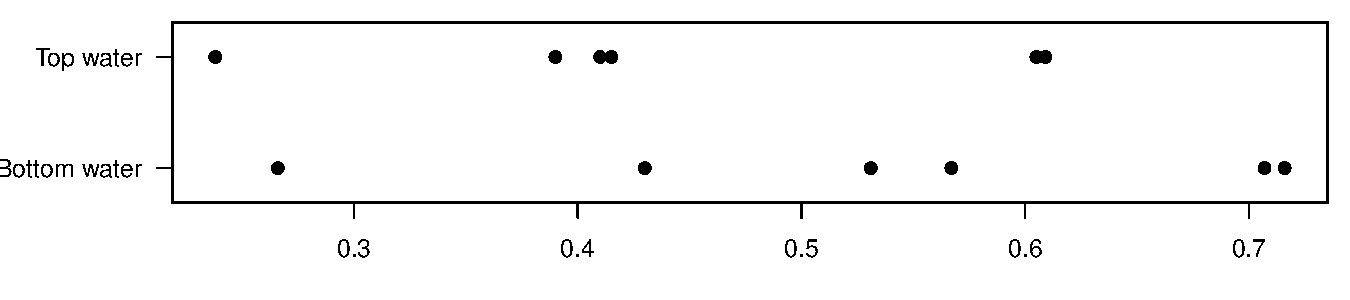
\includegraphics[scale=.5]{ch9_dotplot2.pdf}
\end{center}
%bot=scan(text=".430 .266 .567 .531 .707 .716");
%top=scan(text=".415 .238 .390 .410 .605 .609");
%pdf("ch9_dotplot2.pdf",height=2,width=9);
%par(mai=c(.5,1,0,0)+.1,omi=c(0,0,0,0)+.05,xpd=TRUE,las=1);
%stripchart(list(bot,top),pch=19,at=1:2/3,ylim=c(0.25,.75),group.names=list("Bottom water","Top water"))
%dev.off();
\end{frame}

\begin{frame}{Problem}

We want to test the null hypothesis $H_0: \mu_1-\mu_2=0$ against an alternative $H_0:\mu_1-\mu_2>0$ based on the data:

\begin{center}
\begin{tabular}{l|cccccc}
Location & 1 & 2 & 3 & 4 & 5 & 6 \\ \hline
Bottom water ($X_i$) &
.430 & .266 & .567 & .531 & .707 & .716 \\ \hline
Surface water ($Y_i$) &
.415 & .238 & .390 & .410 & .605 & .609 \\ \hline
%Difference &.015 & .028 & .177 & .121 & .102 & .107
\end{tabular}
\end{center}

\pause It may seem natural to treat this as a two-sample problem: We could calculate $\overline X=.536$, $S_1=.171$, $\overline Y=.444$, and $S_2=.142$:
\pause\begin{align*}
T &= \frac{\overline X-\overline Y-\Delta_0}{\sqrt{\frac{S_1^2}m+\frac{S_2^2}n}}
\uncover<4->{= \frac{.536-.444-0}{\sqrt{\frac{(.171)^2}6+\frac{(.142)^2}6}} }
\uncover<5->{\approx 1.0\\ }
\uncover<6->{\nu &= \left(\frac{S_1^2}{m}+\frac{S_2^2}n\right)^2 \div \left(\frac{(S_1^2/m)^2}{m-1}+\frac{(S_2^2/n)^2}{n-1}\right) }
\uncover<7->{= 9.7 \approx 10 \\}
\uncover<8->{P &= P(T>1.0) }
\uncover<9->{= .170}
\end{align*}
\uncover<10->{However, this method would be \textit{incorrect} because the two samples are not independent of each other!}
\end{frame}


\begin{frame}{Paired t Test}
To test a difference in means between the two normal populations, given a random sample of pairs $(X_1,Y_1), \dots, (X_n,Y_n)$, the correct procedure is to use the \emph{paired t test}:

\pause \vspace{.2cm}
To perform the paired t test, take the differences $D_i=X_i-Y_i$ between corresponding observations in each pair and then perform a one-sample t test on the resulting differences $D_i$.

\pause \begin{block}{}
\begin{tabular}{c|c|c}
Test Statistic & Alternative hypothesis & Rejection region \\ \hline
\multirow{3}{*}{$\displaystyle T=\frac{\overline D-\Delta_0}{S_D/\sqrt{n}}$} & $H_a: \mu_1-\mu_2>\Delta_0$ & $T>t_{\alpha,\nu}$ \\
& $H_a: \mu_1-\mu_2<\Delta_0$ & $T<-t_{\alpha,\nu}$ \\
& $H_a: \mu_1-\mu_2\neq\Delta_0$ & $|T|>t_{\alpha/2,\nu}$\\
\end{tabular}
\end{block}
\pause Here $S_D$ is the sample standard deviation of the differences $D_1,\dots,D_n$, and $\nu=n-1$. If $n$ is large, say $n>40$, then the assumption that the populations are normal may be dropped.

\end{frame}

\begin{frame}{Example}
\begin{block}{}
Does the data provide significant evidence the mean zinc concentration in bottom water exceeds that of surface water?
\end{block}

\begin{center}
\begin{tabular}{l|cccccc}
Location & 1 & 2 & 3 & 4 & 5 & 6 \\ \hline
Bottom water ($X_i$) &
.430 & .266 & .567 & .531 & .707 & .716 \\ \hline
Surface water ($Y_i$) &
.415 & .238 & .390 & .410 & .605 & .609 \\ \hline
Difference ($D_i$) &.015 & .028 & .177 & .121 & .102 & .107
\end{tabular}
\end{center}

\pause We are testing $H_0: \mu_1-\mu_2=0$ against the alternative $H_a: \mu_1-\mu_2>0$. \pause We calculate $\overline D = .0917$, $\overline S=.0607$, so
\begin{align*}
T&=\frac{\overline D-\Delta_0}{S/\sqrt{n}}
\uncover<4->{= \frac{.0917-0}{.0607/\sqrt{6}} }
\uncover<5->{=3.7}
\end{align*}
\uncover<6->{This gives a P-value of $P=P(T>3.7)=.007$. }
\uncover<7->{Thus the data provides highly significant evidence that the mean zinc concentration in bottom water exceeds that of surface water.}
\end{frame}

\begin{frame}{Paired t Confidence Interval}
Again suppose we have two normal populations with means $\mu_1$ and $\mu_2$ respectively, and we wish to construct a confidence interval for $\mu_1-\mu_2$ based on a random sample of pairs $(X_1,Y_1), \dots, (X_n,Y_n)$. 

\pause
\vspace{.2cm}
We form the differences $D_i=X_i-Y_i$ and then simply construct the one-sample t confidence interval based on the $D_i$'s:

\pause
\begin{block}{}
Given paired data from two samples, a $100(1-\alpha)\%$ confidence interval for $\mu_1-\mu_2$ is given by
$$\overline D \pm \frac{t_{\alpha/2,n-1}S_D}{\sqrt{n}}$$
\end{block}

\pause
If $n$ is large, say $n>40$, then the assumption that the populations are normal may be dropped. \end{frame}

\begin{frame}{Example}
\begin{block}{}
Based on the given data, find a 95\% confidence interval for the difference in mean zinc concentration in bottom water vs. surface water.
\end{block}

\begin{center}
\begin{tabular}{l|cccccc}
Location & 1 & 2 & 3 & 4 & 5 & 6 \\ \hline
Bottom water ($X_i$) &
.430 & .266 & .567 & .531 & .707 & .716 \\ \hline
Surface water ($Y_i$) &
.415 & .238 & .390 & .410 & .605 & .609 \\ \hline
Difference ($D_i$) &.015 & .028 & .177 & .121 & .102 & .107
\end{tabular}
\end{center}

\pause Here we have $\overline D = .0917$, $\overline S=.0607$, and $t_{\alpha/2,\nu}=t_{.025,5}=2.571$, \pause so the 95\% confidence interval is given by
\begin{align*}
\overline D \pm \frac{t_{\alpha/2,\nu}S_D}{\sqrt{n}} 
\uncover<4->{&= .0917 \pm  \frac{(2.571)(.0607)}{\sqrt{5}}\\}
\uncover<5->{&= .0917 \pm .0698}
\end{align*}

\end{frame}

\begin{frame}{Large-Sample z Test for Equality of Two Proportions}
Suppose proportion $p_1$ of one population has a certain characteristic, while proportion $p_2$ of a second population does. 

\pause
\vspace{.2cm}We want to test the hypothesis $H_0: p_1=p_2$ based on a random sample of $m$ individuals from the first population and $n$ individuals from the second.

\pause
\vspace{.2cm}Given sample proportions $\hat p_1=\frac X m$ and $\hat p_2=\frac Y n$, the  \emph{z test} is 

\begin{block}{}
\begin{tabular}{c|c|c}
Test Statistic & Alternative hyp. & Rejection region \\ \hline
\multirow{3}{*}{$\displaystyle Z=\frac{\hat p_1-\hat p_2}{\sqrt{\hat p(1-\hat p)\left(\frac1m+\frac1n\right)}}$} & $H_a: p_1>p_2$ & $Z>z_{\alpha}$ \\
& $H_a: p_1<p_2$ & $Z<-z_{\alpha}$ \\
& $H_a: p_1\neq p_2$ & $|Z|>z_{\alpha/2}$\\
\end{tabular}
\end{block}

\pause
Here $\hat p=\frac{X+Y}{m+n}$ is the \emph{pooled sample proportion}.

\pause
\vspace{.2cm}
This is a large-sample test, appropriate only if $X, m-X, Y, n-Y$ are all at least 10.
\end{frame}

\begin{frame}{Example}
\begin{block}{}
An article reported that of 549 study participants who
regularly used aspirin after being diagnosed with colorectal cancer, there were 81
colorectal cancer-specific deaths, whereas among 730 similarly diagnosed individuals who did not subsequently use aspirin, there were 141 colorectal cancer-specific
deaths\footnotemark. Does this data suggest that the regular use of aspirin after diagnosis will
decrease the incidence rate of colorectal cancer-specific deaths?
\end{block}

\pause Here we want to test the null hypothesis $H_0: p_1=p_2$ against the alternative $H_a: p_1<p_2$. \pause We have $m=549$, $n=730$, $\hat p_1=\frac{81}{549}$, $\hat p_2=\frac{141}{730}$, $\hat p=\frac{81+141}{549+730}$.
\pause \begin{align*}
Z&=\frac{\hat p_1-\hat p_2}{\sqrt{\hat p(1-\hat p)\left(\frac1m+\frac1n\right)}} 
\uncover<5->{=  -2.13 \\}
\uncover<6->{P&=P(Z<-2.13)}
\uncover<7->{=.0166}
\end{align*}

\footnotetext{``Aspirin Use and Survival After Diagnosis of Colorectal Cancer" (J. of
the Amer. Med. Assoc., 2009: 649--658)}
\end{frame}

\begin{frame}{z Confidence Interval for Difference of Two Proportions}
Suppose proportion $p_1$ of one population has a certain characteristic, while proportion $p_2$ of a second population does. 

\pause\vspace{.2cm}
Assume we have a random sample of $m$ individuals from the first population and $n$ individuals from the second, and let $\hat p_1=\frac X m$ and $\hat p_2=\frac Y n$ be the sample proportions.

\pause\begin{block}{}
An approximate $100(1-\alpha)\%$ confidence interval for $p_1-p_2$ is
$$\hat p_1-\hat p_2 \pm z_{\alpha/2}\sqrt{\frac{\hat p_1(1-\hat p_1)}m+\frac{\hat p_2(1-\hat p_2)}n}$$
\end{block}

\pause Note that the pooled sample proportion $\hat p$ does \textit{not} appear in the confidence interval for a difference of two proportions.

\pause
\vspace{.2cm}
Again this is a large-sample procedure, appropriate only if $X, m-X, Y, n-Y$ are all at least 10.
\end{frame}

\begin{frame}{Example}
\begin{block}{}
Recall the data from the colorectal cancer study: 81 deaths out of 549 participants who took aspirin, and 141 out of 730 who did not take aspirin. Find an approximate 95\% confidence interval for the difference between the two proportions.
\end{block}

\pause We have $m=549$, $n=730$, $\hat p_1=\frac{81}{549}$, $\hat p_2=\frac{141}{730}$; \pause  an approximate 95\% confidence interval is given by

\begin{align*}
&\hat p_1-\hat p_2 \pm z_{\alpha/2}\sqrt{\frac{\hat p_1(1-\hat p_1)}m+\frac{\hat p_2(1-\hat p_2)}n}\\
&=  -.046 \pm  .041
\end{align*}
\end{frame}

%\begin{frame}{F Test for Equality of Variances}

%\end{frame}

\begin{frame}{Summary}

\vspace{-.6cm}
\renewcommand*{\arraystretch}{1.4}
\begin{center}
\begin{tabular}{|p{5cm}|l|}
\hline
Two-sample z C.I.\@ for $\mu_1-\mu_2$  & $\overline{X} - \overline{Y} \pm z_{\alpha/2}\sqrt{\frac{\sigma_1^2}m+\frac{\sigma_2^2}n}$ \\ \hline
Two-sample t C.I.\@ for $\mu_1-\mu_2$ & $\overline{X} - \overline{Y} \pm t_{\alpha/2,\nu}\sqrt{\frac{S_1^2}m+\frac{S_2^2}n}$ \\ \hline
Paired t C.I.\@ for $\mu_1-\mu_2$ & 
$\displaystyle\overline D \pm \frac{t_{\alpha/2,n-1}S_D}{\sqrt{n}}$ \\ \hline
Approximate C.I.\@ for $p_1-p_2$ & $\hat p_1-\hat p_2 \pm z_{\alpha/2}\sqrt{\frac{\hat p_1(1-\hat p_1)}m+\frac{\hat p_2(1-\hat p_2)}n}$ \\ \hline
\end{tabular}
\end{center}

\vspace{-.3cm}
\begin{center}
\begin{tabular}{|p{1.2in}|l|l|} \hline
Test & Null Hypothesis & Test Statistic  \\ \hline
Two-sample z test & $H_0: \mu_1-\mu_2=\Delta_0$ &$Z=\frac{\overline X-\overline Y-\Delta_0}{\sqrt{\frac{\sigma_1^2}m+\frac{\sigma_2^2}n}}$  \\ \hline
Two-sample t test & $H_0: \mu_1-\mu_2=\Delta_0$ & $T=\frac{\overline X-\overline Y-\Delta_0}{\sqrt{\frac{S_1^2}m+\frac{S_2^2}n}}$  \\ \hline
Paired t test & $H_0: \mu_1-\mu_2=\Delta_0$ & $T=\frac{\overline D-\Delta_0}{S_D/\sqrt n}$  \\ \hline
Approximate z test for proportions & $H_0: p_1=p_2$ & $Z=\frac{\hat p_1-\hat p_2}{\sqrt{\hat p(1-\hat p)\left(\frac1m+\frac1n\right)}}$  \\ \hline
\end{tabular}
\end{center}

\end{frame}

\end{document}
